%%%%%%%%%%%%%%%%%%%%%%%%%
%% Header for standard beamer presentation
%%
%%  PresentationHeader.tex
%%
%%%%%%%%%%%%%%%%%%%%%%%%%

\documentclass[english,10pt]{beamer}

%%%%%%%%%%%%%%%%%%%%
%% Include general header where common packages are defined
%%%%%%%%%%%%%%%%%%%%

% general packages without options
\usepackage{amsmath,amssymb,bbm}




%%%%%%%%%%%%%%%%%%%%
%% Idem general commands
%%%%%%%%%%%%%%%%%%%%

%%% Commands

\newcommand{\noun}[1]{\textsc{#1}}


%% Math

% Operators
\DeclareMathOperator{\Cov}{Cov}
\DeclareMathOperator{\Var}{Var}
\DeclareMathOperator{\E}{\mathbb{E}}
\DeclareMathOperator{\Proba}{\mathbb{P}}

\newcommand{\Covb}[2]{\ensuremath{\Cov\!\left[#1,#2\right]}}
\newcommand{\Eb}[1]{\ensuremath{\E\!\left[#1\right]}}
\newcommand{\Pb}[1]{\ensuremath{\Proba\!\left[#1\right]}}
\newcommand{\Varb}[1]{\ensuremath{\Var\!\left[#1\right]}}

% norm
\newcommand{\norm}[1]{\| #1 \|}


% amsthm environments
\newtheorem{definition}{Definition}



%% graphics

% renew graphics command for relative path providment only ?
%\renewcommand{\includegraphics[]{}}






\usetheme{Warsaw}

\setbeamertemplate{footline}[text line]{}
\setbeamercolor{structure}{fg=purple!50!blue, bg=purple!50!blue}

\setbeamercovered{transparent}


% shortened command for a justified frame
\newcommand{\jframe}[2]{\frame{\frametitle{#1}\justify{#2}}}



%%%%%%%%%%%%%%%%%%%%%
%% Begin doc
%%%%%%%%%%%%%%%%%%%%%

\begin{document}



\title{Thesis Progress Meeting}


\author{J.~Raimbault$^{1,2}$}

\institute{$^{1}$G{\'e}ographie-Cit{\'e}s (UMR 8504 CNRS)\\
$^{2}$LVMT (UMR-T 9403 IFSTTAR)}


\date{May 26th 2015
}


%%%%%%%%%%%%%%%%%%%%%%%%%%%%%%%%
\begin{frame}
\titlepage
\end{frame}

%\begin{frame}
%\tableofcontents
%\end{frame}
%%%%%%%%%%%%%%%%%%%%%%%%%%%%%%%%


\section{Projects Organization}

\jframe{Projects Organization (current projects only)}{
   \includegraphics[width=\textwidth,height=0.8\textheight]{figures/orgaProjects}
}



\section{Achieved Work}


\jframe{Achieved Work (by projects)}{
\begin{itemize}
\item Technical Tools : multi-purpose library for current NetLogo utilities. [0.4w]
\item Bibliography : general and specific. [1w]
\item Algorithmic Systematic Review : finished ECTQG paper ; anonymized request (TOR) to contourne scholar restrictions. [0.4w]
\item Synthetic Data Control : model exploration ; Link with Romain \& al. project (Schelling). [0.5w]
\item Stochastic Urban Growth : link between Gibrat and Simon models. [0.5w]
\item Governance : new implementation paradigms (dynamic programming) ; model v3 currently being coded. [0.6w]
\item Scaling Sensitivity : confirmation of structural effect for density-driven indicators ; check on real data by Clementine [0.8w]
\item Epistemological Essay Drafting. [0.4w]
\item Side Projects : Discrepancy ; Transportation Equilibrium Validity. [0.4w]
\end{itemize}
}



\section{Technical Developments}



%%%%%%%%%%%%%%%%%%%%%%%%%%%%%%%%
\jframe{Bibliography}{
\textit{General and more specific bibliography.} Idea : frame case studies/particular situations/generalities etc. recurring in city-transport interactions.

\bigskip

\begin{itemize}
\item ``Classics'' in economy~\cite{anas1998urban}, \cite{Gabaix20042341}
\item Metropolitan Governance : Grand Paris example~\cite{gilli2009paris}
\item Far East Russian new towns (Transsiberian/Baikal-Amour)~\cite{underhill1990soviet} ; possibility of unusual instruments.
\item Idem for South Africa (apartheid-shaped network : statistical control on bottom-up effects) : possibility to work with Solene.
\item French railway : specific historic case, good dataset~\cite{thevenin2013mapping} ; recent LGV question~\cite{zembri2008contribution} ; discussion with Francois.
\end{itemize}

}



%%%%%%%%%%%%%%%%%%%%%%%%%%%%%%%%
\jframe{Governance : MetropolSim Model}{

A toy-model initially proposed by Florent~\cite{lenechet2012}, aimed to explore the role of governance in transportation network evolution, and conditions for emergence of common governance and metropolitan structure. Couples a luti with evolving transportation network.

\medskip

\textit{MetropolSim v2} Refactorization, commenting and implementation improvement (nw extension use e.g.) of v1.9 by Florent. Pb : Using standard network paradigms is far too slow, even by caching shortest paths (due in particular to the large size of explored space when extending transportation newtork), even with very few patches (16)

\medskip

$\rightarrow$ \textit{MetropolSim v3} currently implemented (75\%), with dynamic programming for network management : reasonable execution time with $60^2$ patches.

\medskip

\textit{Next Steps : finish implementation and first explorations for 4th June.} 

}


%%%%%%%%%%%%%%%%%%%%%%%%%%%%%%%%
\jframe{Scaling Sensitivity}{
Exponential Mixture distribution for density in an urban system $d(\vec{x}) = \sum_{i=1}^{N}{d_i(\vec{x})} = \sum_{i=1}^{N}{d_i^0\cdot \exp{\left(\frac{-\norm{\vec{x}-\vec{x}_i}}{r_i}\right)}}$, local probability of presence for amenity $\Pb{a(\vec{x})=1}=f(d(\vec{x}))=\lambda\cdot d(\vec{x})^\beta$.

Indicators defined by $A_i(\theta)=\Eb{\iint_{D(\vec{x}_i,\theta)}{a(\vec{x})d\vec{x}}}$, for city $i$ with density threshold $\theta$.

\smallskip

We compute the expression of scaling exponent $\alpha(\theta)$ for $A_i$ scaling with $P_i$, as a rational fraction in $\theta$ and $\ln{\theta}$.

\smallskip
Numerical application confirms the expression ; same qualitative results with different kernels and various parameter values.
\smallskip

\textbf{Implication : } for that type of indicators, scaling variability is only structural $\rightarrow$ solution to test if a variable only depends on density, without spuriousity problems.
\smallskip

\textit{Next Steps : } Tests on real data (Cl{\'e}mentine) ; sensitivity to kernel ; bi-parameter phase diagram.

}



%%%%%%%%%%%%%%%%%%%%%%%%%%%%%%%%
\jframe{Stochastic Urban Growth}{
Seminal debate on stochastic models of urban growth, in particular Gibrat/Simon \cite{gabaix1999zipf} ; recent pretention of physicists to introduce ``scientific models of the city''~\cite{2014arXiv1401.8200L}.

\smallskip

$\rightarrow$ indeed, most stochastic models of urban growth can be understood as part of a general framework, where models are discrete/continous declination of a same meta-model, and can be linked.

\smallskip

\textbf{Current Results : } \textit{A preferential attachment model with death and birth (Simon model) is in large size limit a Gibrat model where distributions at each time step are entirely determined (moments ar any orders are deterministic).
Reciprocally, the discretization of a Gibrat model produces a preferential attachment where fixation probability function is given by Gibrat distribution parameters.
}

\smallskip

\textit{Next steps : } Link with Favaro-Pumain, with generalized preferential attachment ; classification of models ; formulation of ``missing'' models (ex equivalent of Favaro-Pumain) ; concrete applications (ex. exact determination of scaling exponent in a Gibrat using results on PrefAtt~\cite{yamasaki2006preferential}).

}



%%%%%%%%%%%%%%%%%%%%%%%%%%%%%%%%
\jframe{Synthetic Data Control}{
Preferential Attachment spatialized (through diffusion) model (note : similar to an unexplored shady model by Batty~\cite{batty2006hierarchy}), initially aimed to generate density patterns that would be used as initial conditions for a coupled network-density model : possibility of statistical control on meta-parameters and accurate expected effects.

$\rightarrow$ analog demarch as in a project by Romain et al., integration in the project (density generator and general methodological framework)

\textbf{Calibration :} European 200m grid, morphological indicators~\cite{le2015forme} computed in 100km squares, compared with model outputs. First grid exploration, confirms the need of fine tuning : GA or finer targeted grid. \textit{Q : obtain a grid certificate ?}


\hfill
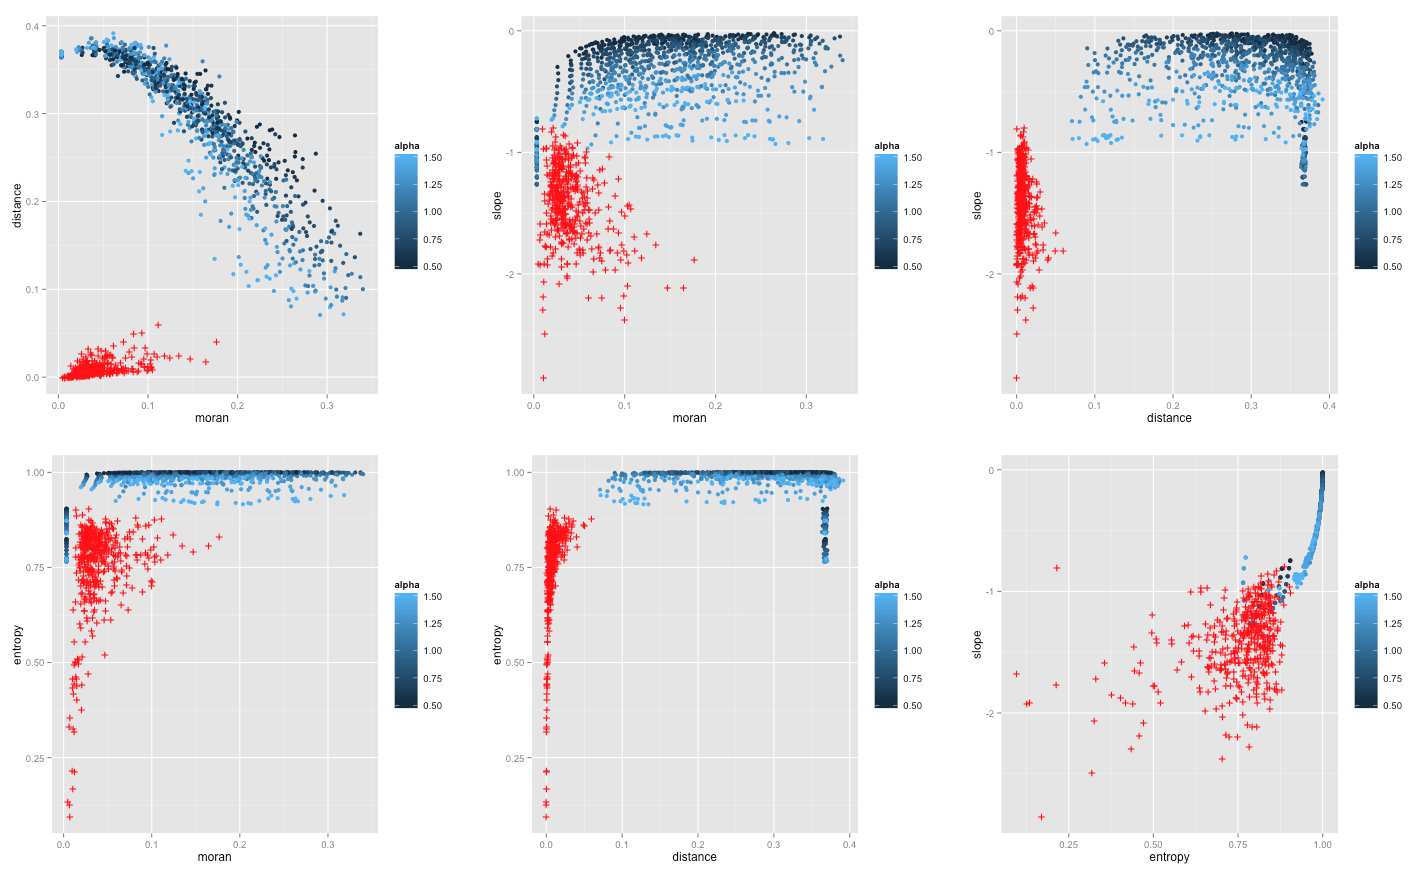
\includegraphics[width=0.5\textwidth,height=0.3\textheight]{figures/alpha_withreal}
\hfill\hfill


}


%%%%%%%%%%%%%%%%%%%%%%%%%%%%%%%%
\jframe{Epistemological Essay}{
Reflexion on the importance of mutually respecting interactions between disciplines and the difficulty of multidisciplinarity. No theoretical pretention but recurrent experiences/examples motivate it.

\bigskip

In particular :

\begin{itemize}
\item \textit{Physics reinvents geography} : arrogance of some physicists regarding geography, felt in many papers and recent seminars.
\item \textit{Economic Geography vs Geographical Economics} : similar ``conflict''~\cite{marchionni2004geographical}
\item \textit{Agent-based modeling in economy} : scientific misunderstanding by most economists~\cite{farmer2009economy}
\item \textit{Quantitative Finance} : conflict between advanced mathematical approaches and empirical physics/complex systems paradigms.
\end{itemize}



\bigskip



\textit{Next Steps : } Decent draft (not enough solid for now).

}




%%%%%%%%%%%%%%%%%%%%%%%%%%%%%%%%
\begin{frame}[allowframebreaks]
\frametitle{References}
\bibliographystyle{apalike}
\bibliography{/Users/Juste/Documents/ComplexSystems/CityNetwork/Biblio/Bibtex/CityNetwork}
\end{frame}
%%%%%%%%%%%%%%%%%%%%%%%%%%%%%%%%


\end{document}